\chapter{La machine synchrone}

\section{La machine synchrone à entrefer constant, en régime symétrique
d'ordre direct}

	\subsection{Constitution - Rappels}
	Au niveau du stator, pas de grande différence avec celui du moteur 
	asynchrone : enroulements ouverts constituant les trois phases. Le 
	rotor est lisse : entrefer constant. Il est cependant muni d'encoches 
	dans lesquelles sont placés les enroulement d'excitation parcouru en 
	régime par un courant \textbf{continu}.\\
		\begin{wrapfigure}[12]{l}{5.3cm}
		\vspace{-5mm}
	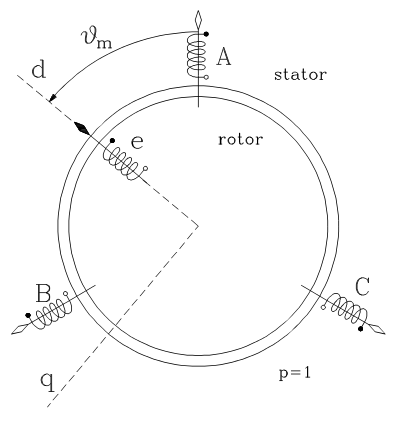
\includegraphics[scale=0.3]{ch7/image1.png}
	\captionof{figure}{ }
	\label{fig:schema7}
	\end{wrapfigure}	
	Le but est qu'à l'aide de courants statorique équilibré à fréquence 
	$\omega$, on crée un champ tournant à vitesse $\omega$. Ce champ 
	tournant entraîne le rotor à vitesse
	\begin{equation}
	\Omega = \dfrac{\omega}{p}
	\end{equation}
	Le seul courant pouvant circuler dans l'enroulement d'excitation $e$ 
	est du à une source extérieure, ici continue.\\

	Ci-contre, les trois enroulement statorique et l'enroulement rotorique 
	décalé de $\vartheta_m$ par rapport à l'axe de la phase $A$. On dirige 
	l'axe de l'enroulement $e$ selon la maximum d'induction qu'il crée : 
	l'axe longitudinal $d$. L'axe transversal $q$ est décalé de 90$^\circ$ 
	en avant par rapport à lui.\\
	On peut écrire pour la machine de la \autoref{fig:schema7} :
	\begin{equation}
	\left(\begin{array}{c}
	\Psi_A\\
	\Psi_B\\
	\Psi_C\\
	\Psi_D
	\end{array}\right) = \left(\begin{array}{cccc}
	L_A & M_{AB} & M_{AB} & M^M\cos\theta\\
	M_{AB} & L_A & M_{AB} & M^M\cos(\theta-\frac{2\pi}{3})\\
	M_{AB} & M_{AB} & L_A & M^M\cos(\theta+\frac{2\pi}{3})\\
	M^M\cos\theta & M^M\cos(\theta-\frac{2\pi}{3}) & (\theta+\frac{2\pi}{3}) & L_e
	\end{array}\right)\left(\begin{array}{c}
	i_A\\
	i_B\\
	i_C\\
	i_e
	\end{array}\right)
	\end{equation}
	On observe la même inductance mutuelle entre les enroulements statoriques 
	et rotorique. De façon condensée :
	\begin{equation}
	[\Psi_{Ae}] = [L_{Ae}][i_{Ae}]
	\end{equation}
	L'inductance propre d'une phase statorique vaut (p7, ch3)\footnote{Inductance 
	de dispersion + inductance de magnétisation}
	\begin{equation}
	L_A = l_a + N^2\mathcal{P}_m
	\end{equation}
	L'inductance mutuelle entre des phases statoriques vaut
	\begin{equation}
	M_{AB} = l_A' - \frac{1}{2}N^2\mathcal{P}_m
	\end{equation}
	L'inductance propre de l'enroulement d'excitation vaut 
	\begin{equation}
	L_e = l_e + N_e^2 \mathcal{P}_m
	\end{equation}
	L'inductance mutuelle entre la phase $A$ du stator et l'enroulement $e$ du 
	rotor vaut
	\begin{equation}
	M_{Ae} = NN_e\mathcal{P}_m\cos\theta = M^M\cos\theta
	\end{equation}
	avec $M^M = NN_E\mathcal{P}_m$.\\
	Compte-tenu de ces expressions, on peut tout remplacer dans la matrice pour 
	obtenir $\Psi_A, \dots$, expressions non reprises ici. 
	
	
	\subsection{Le régime symétrique d'ordre direct}
	Lorsqu'elle fonctionne en générateur, elle porte le doux nom d'\textit{alternateur} 
	qui est bien une source de puissance électrique.
	
		\subsubsection{Fonctionnement à vide d'un alternateur}
		On ouvre le stator $i_A=i_B=i_C=0$ et on excite le rotor par un courant 
		continu $I_e=I_E$. Pour la rotation, on considère $\theta=\theta_0+\omega t$ 
		avec $\Omega_r = \omega/p$.\\
		L'expression de $\Psi_e$ sous ces conditions (en déballant la matrice, ahah!) :
		\begin{equation}
		\Psi_e = l_ei_e + N_e^2\mathcal{P}_mi_e =\ cste
		\end{equation}
		La tension appliquée à l'excitation est alors forcément constante :
		\begin{equation}
		v_e = r_ei_e + \underbrace{\dfrac{d\Psi_e}{dt}}_{=0}
		\end{equation}
		Les flux dans chacune des phases statoriques sont donnés par :
		\begin{equation}
		\begin{array}{ll}
		\Psi_A &= NN_e\mathcal{P}_m\cos\theta\ i_e\\
		\Psi_B &= NN_e\mathcal{P}_m\cos(\theta-\frac{2\pi}{3})\ i_e\\
		\Psi_C &= NN_e\mathcal{P}_m\cos(\theta+\frac{2\pi}{3})\ i_e\\
		\end{array}
		\end{equation}
		Il est possible d'obtenir ces flux de deux autres façons (voir paragraphe 5.1.3 et 
		\autoref{fig:schema_p}) :
		\begin{enumerate}
		\item Par projection sur l'axe de chacune des phases du vecteur $\overline{\Psi}$ 
		(amplitude $NN_e\mathcal{P}_mI_e$ et déphasage de $\theta=\theta_0+\omega t$ par 
		rapport à la phase $A$)
		\item Déduit du système direct de phaseurs $\sqrt{2}\overline{\Psi} = NN_e
		\mathcal{P}_mI_ee^{j\theta}$.
		\end{enumerate}
		
		\begin{center}
		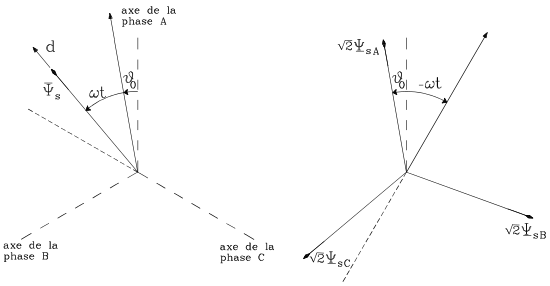
\includegraphics[scale=0.4]{ch7/image2.png}
		\captionof{figure}{ }
		\label{fig:schema_p}
		\end{center}
		\newpage
		
		\begin{wrapfigure}[9]{l}{4cm}
		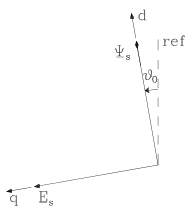
\includegraphics[scale=0.5]{ch7/image3.png}
		\captionof{figure}{ }
		\end{wrapfigure}	
		On peut voir sur \autoref{fig:schema_p} qu'en $t=0$ les deux diagramme se 
		superposent pour la phase $A$. En parlant de la phase $A$, voici la tension 
		qu'elle engendre (on considère que l'alignement de $\underline{\Psi}_s$ est 
		aussi l’alignement de l'axe longitudinal $d$ (en $t=0+k2\pi/\omega$)) :
		\begin{equation}
		v_A = \dfrac{d\Psi_A}{dt}\quad \text{ ou }\quad \underline{E}_s = j\omega
		\underline{\Psi}_s
		\end{equation}
		On peut représenter ça en diagramme des phaseurs (flux/tension efficace). Si 
		$\underline{\Psi}_s$ est aligné sur $d$, la tension $\underline{E}_s$ étant 
		déphasée de 90$^\circ$ elle est alignée selon $q$.\\
		
		On peut montrer qu'un alternateur à vide est une source de trois tensions 
		sinusoïdale symétrique d'ordre direct et de valeur efficace :
		\begin{equation}
		\begin{array}{ll}
		\underline{E_s} &= \omega NN_e\mathcal{P}_m \frac{I_e}{\sqrt{2}}\\
		&= \omega\dfrac{L_m}{\mu_p}\dfrac{I_e}{\sqrt{2}}\\
		&= \dfrac{X_m}{\mu_p\dfrac{I_e}{\sqrt{2}}}
		\end{array}
		\label{eq:Egg}
		\end{equation}
		où $\mu = \dfrac{\frac{3}{2}N}{N_e}$ est le rapport de transformation de 
		Potier et $X_m = \omega L_m$ est la réactance de magnétisation. Le phaseur
		$\underbrace{E}_s$ est ainsi la composante symétrique directe du système de 
		trois tensions, aligné sur l'axe $q$.
		
		
		\subsubsection{Fonctionnement sous charge symétrique}
		Si les impédances de chaque phases sont égales, les courants débités 
		formeront toujours un système symétrique d'ordre direct de pulsation 
		$\omega$.\\
		
		On passe en \textbf{moteur} si le déphasage du courant absorbé sur la tension 
		appliquée est, en valeur absolue, inférieur à $90^\circ$.\footnote{??}. Soit 
		le système de courants statoriques (absorbés) :
		\begin{equation}
		\begin{array}{ll}
		i_A &= I\sqrt{2}\cos(\omega t + \xi_I)\\
		i_B &= I\sqrt{2}\cos(\omega t + \xi_I - \frac{2\pi}{3})\\
		i_C &= I\sqrt{2}\cos(\omega t + \xi_I+\frac{2\pi}{3})				
		\end{array}
		\end{equation}
		avec un courant rotorique $i_e=I_e$ constant. Les courants statoriques 
		créent un champ tournant à vitesse $\omega$. Prouvons que le flux total 
		enserré par l'enroulement d'excitation est constant. Après quelques 
		opérations trigonométriques, on trouve
		\begin{equation}
		\Psi_e = l_eI_e + N_e^2\mathcal{P}_mI_e + NN_e\mathcal{P}_mI\sqrt{2}
		\frac{3}{2}\cos(\theta_0-\xi_I)
		\end{equation}
		Il s'agit d'une constante : ceci prouve que le flux coupé par $e$ est bien 
		constant dans le temps car le champ tournant est fixe par rapport au rotor 
		(vu qu'ils tournent de façon synchrone, il le voit constant). Du coup :
		\begin{equation}
		v_e = r_ei_e
		\end{equation}
		De façon similaire, le flux totalisé coupé par l'enroulement $A$ vaut :
		\begin{equation}
		\Psi_A = li_a + \frac{3}{2}N^2\mathcal{P}_mi_A + NN_e\mathcal{P}_m\cos
		(\omega t+ \theta_0)I_e
		\end{equation}
		On trouve pareil pour $\Psi_B$ et $\Psi_C$ : on peut en déduire une 
		composante symétrique d'ordre direct de ces trois flux :
		\begin{equation}
		\underline{\Psi} = \underline{\Psi}_d+\underline{\Psi}_I+\underline{\Psi}_s
		\end{equation}
		avec $\underline{\Psi}_d$ le flux de dispersion statorique qui ne traverse 
		pas l'entrefer, $\underline{\Psi}_i$ le flux de réaction d'induit (flux d'entrefer 
		du aux courants statoriques), $\underline{\Psi}_s$ le flux d’entrefer 
		du à l'enroulement d'excitation et $\underline{\Psi}_r = \underline{\Psi}_I
		+\underline{\Psi}_s$ le flux d'entrefer \textbf{résultant} $\propto$ 
		l'induction dans l'entrefer.\\
		
		La composante symétrique d'ordre direct des tensions statorique a pour 
		valeur\footnote{??}
		\begin{equation}
		\underline{V} = r\underline{I}+jx\underline{I}+jX_m\underline{I}+\underline{E_s}
		\label{eq:VcompoStato}
		\end{equation}
		On a posé 
		\begin{equation}
		\underline{E_s} = j\omega\underline{\Psi_s} = j\dfrac{X_m}{\mu_P}\dfrac{I_e}{
		\sqrt{2}}e^{j\theta_0}
		\end{equation}
		Ce phaseur représente la fem \textbf{synchrone} : la tension engendrée par le 
		courant d'excitation dans les enroulements d'armature. Par le th. de Thévenin, 
		il vaut la fem à vide.\\
		On peut également defini un phaseur "courant d'exitation" :
		\begin{equation}
		\underline{I_e} = \dfrac{I_e}{\sqrt{2}}e^{j\theta_0}
		\end{equation}
		n'ayant aucune réalité physique mais étant aligné sur le même axe que 
		$\underline{\Psi_s}$ on peut écrire
		\begin{equation}
		\underline{E_s} = j\dfrac{X_m}{\mu_P}\underline{I_e}
		\end{equation}
		en posant $X_m = \frac{3}{2}\omega N^2\mathcal{P}_m$, la réactance de 
		magnétisation. On trouve :
		\begin{itemize}
		\item[$\bullet$] $x=\omega l$ la réactance de dispersion (peu influencée par 
		l'état magnétique de la machine)
		\item[$\bullet$] $r$ la résistance d'une phase statorique (souvent négligeable)
		\item[$\bullet$] $\underline{z} = r+jx$ l'impédance de dispersion
		\item[$\bullet$] $\underline{Z_s} = \underline{z}+jXM$ l'impédance synchrone.
		\end{itemize}\ 
		
		
		\begin{wrapfigure}[11]{l}{6.2cm}
		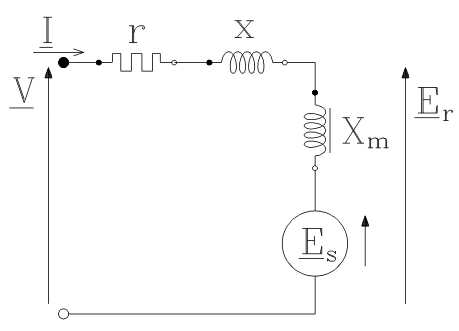
\includegraphics[scale=0.4]{ch7/image4.png}
		\captionof{figure}{ }
		\label{eq:Waw}
		\end{wrapfigure}			
		On peut alors définir
		\begin{equation}
		\begin{array}{ll}
		\underline{E_r} &= j\omega\underline{\Psi_r}\\
		&= j \omega (\underbrace{\Psi}_I+\underline{\Psi}_s)\\
		&= jX_m\underline{I}+\underline{E_s}
		\end{array}
		\end{equation}
		où l'on retrouve le flux d'entrefer dû aux enroulements statoriques et le flux 
		d'entrefer dû à l'enroulement d'excitation.\\
		$\underline{E_r}$ est la \textbf{fem résultante}, proportionnelle au flux résultant 
		dans l'entrefer : normal, c'est lui qui \textbf{fixe l'état magnétique de la machine.}
		A l'aide de \autoref{eq:VcompoStato} on peut obtenir le schéma équivalent ci-contre.
		
		\newpage
		\subsubsection{Calcul du courant d'excitation (fonctionnement moteur)}
		\begin{wrapfigure}[11]{l}{5.5cm}
		\vspace{-5mm}
		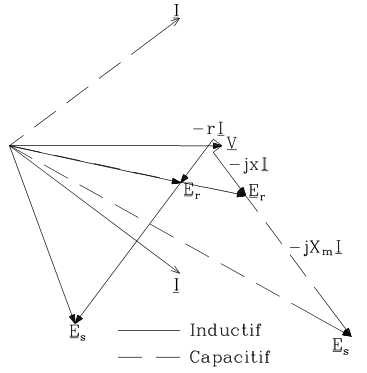
\includegraphics[scale=0.4]{ch7/image6.png}
		\captionof{figure}{ }
		\end{wrapfigure}			
		Si l'on a $\underline{V},\underline{I}$, on peut se demander quel est le courant 
		d'excitation correspondant. A partir de l'extrémité de $\underline{V}$ on peut 
		tracer\footnote{Comment? Le $-jI$ donne qqch de $\perp \underline{I}$ no?}
		\begin{equation}
		-(r+jx)\underline{I}
		\end{equation}
		Pour obtenir $\underline{E_r}$. Ensuite : 
		\begin{equation}
		-jX_m\underline{I}
		\end{equation}
		pour obtenir $\underline{E_s}$. La valeur $I_e$ se déduit de $E_s$.\\
		
		\vspace{1cm}
		
		\subsubsection{Fonctionnement en alternateur}
		Il "suffit" de considérer un courant \textbf{débité} $-\underline{I}$ pour 
		respecter les conventions. Ci-dessous à droite, la figure pour déterminer $E_s$ et 
		$I_e$.
		\begin{center}
		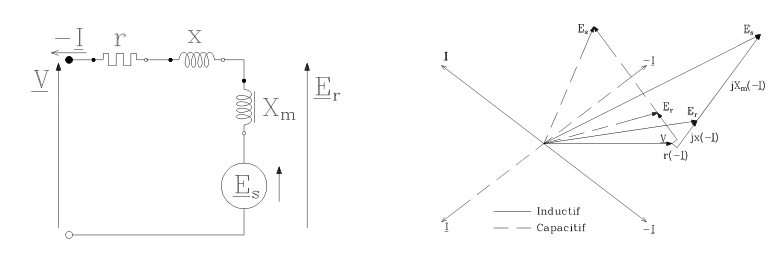
\includegraphics[scale=0.5]{ch7/image5.png}
		\captionof{figure}{ }
		\label{fig:SchEqGen}
		\end{center}
		
	\subsection{La mesure des paramètres de la machine à entrefer constant}
	\subsubsection{Caractéristique à vide}
			\begin{wrapfigure}[13]{l}{4.5cm}
		\vspace{-5mm}
		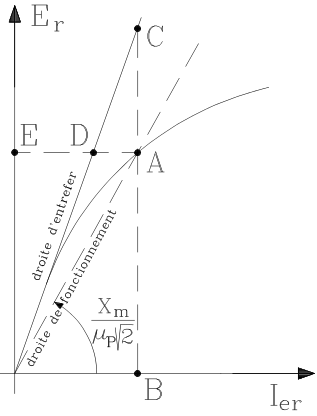
\includegraphics[scale=0.4]{ch7/image7.png}
		\captionof{figure}{ }
		\label{fig:CaracVide}
		\end{wrapfigure}		
	La perméance $\mathcal{P}_m$ et la réactance $X_m$ sont influence par la saturation. 
	Supposons que $X_m$ soit fonction du flux résultant,ou en fonction de $E_r$ ou encore 
	du courant d'excitation 
	résultant $\underline{I}_{er} = \underline{I}_e + \mu_p\underline{I}$.\\
	
	Ainsi, si on connaît $E_r = f(I_{er})$ (soit la fem résultante en fonction du courant 
	d'excitation résultant) on peut retrouver $X_m$ pour un point $A$ : la pente joignant 
	l'origine au point $A$ valant (voir \autoref{eq:Egg})
	\begin{equation}
	\dfrac{X_m}{\mu_P\sqrt{2}}
	\end{equation}
	La courbe de la \autoref{fig:CaracVide} est la \textbf{caractéristique à vide} tracée pour 
	une vitesse de rotation donnée. Elle donne la variation de tension aux bornes en fonction 
	du courant d'excitation à vide car $\underline{V}=\underline{E_r}, I_e = I_{er}$.\\
	
	Cette caractéristique est "assez linéaire" comme l'entrefer est assez grand : il 
	s'agit de la \textit{droite d'entrefer}.
	
		\subsubsection{Choix de la base rotorique (pour $I_e$}
		Résultat à admettre : base d'excitation :
		\begin{equation}
		I_{eB} = \mu_P\sqrt{2}I_B
		\end{equation}
		L'équation \autoref{eq:Egg} devient alors 
		\begin{equation}
		\dfrac{E_s}{V_b} = \dfrac{\dfrac{X_m}{\mu_P\sqrt{2}}}{Z_B}\dfrac{I_e}{I_B} = 
		\dfrac{X_m}{Z_B}\dfrac{I_e}{\mu_P\sqrt{2}I_B}
		\end{equation}
		\begin{center}
		Partie à connaître ? Pas super drôle.
		\end{center}
		
		\subsubsection{Droite de court-circuit}
		Soit un court circuit triphasé aux bornes de la machine. On a donc 
		\begin{equation}
		0 = \underline{V} = z \underline{I_{cc}} + \underline{E_r}
		\end{equation}
		Avec le schéma de la \autoref{fig:SchEqGen}, on peut calculer le courant 
		\begin{equation}
		\underline{I_{cc}} = -\dfrac{\underline{E_s}}{\underline{z}+jX_{m,ns}}
		\end{equation}
		Avec \autoref{eq:Waw}, on peut écrire
		\begin{equation}
		\underline{I_{cc}} = -\dfrac{jX_{m,ns}}{\underline{z}+jX_{m,ns}}\dfrac{\underline{I_e}}{
		\mu_P}
		\end{equation}
		La relation $I_cc = f(I_e)$ est linéaire : c'est la \textbf{droite de 
		court-circuit}	dont la pente vaut (on isole et on prend le module) :
		\begin{equation}
		\dfrac{1}{\sqrt{2}\mu_P}\dfrac{X_{m,ns}}{x+X_{m,ns}}
		\end{equation}
		En pratique, on utilise souvent le \textbf{rapport de cour-circuit} (cf. labo).
		
		
		\subsubsection{Caractéristique en déwatté - Triangle de POTIER}
		On souhaite tracer la caractéristique en déwatté inductif, alternateur : 
		\begin{equation}
		V = f(I_e)\quad \text{ pour } (-I) =\ cste\quad \text{et } \phi = +\frac{\pi}{
		2}\quad (\cos\phi=0)
		\end{equation}
		Si $r=0$, $\underline{V}, \underline{E_r}, \underline{E_s}$ sont alignées selon 
		l'axe $q$ et les courants $\underline{I},\underline{I_e}, \underline{I_{er}}$ 
		selon $d$. Cela permet, via le diagramme, de calculer la tension $V$ 
		correspondant à $I_e$ pour une valeur donnée de $I$ sachant que
		\begin{equation}
		I_{er} = I_e-\mu_PI\sqrt{2}
		\end{equation}
		
		\begin{center}
		?? (Page 22) ?? $\Rightarrow$ Qu'est ce qu'on déduit de 7.1-17?
		\end{center}
		
		La caractéristique en déwatté (pour $I$ donné) se déduit de la caractéristique 
		à vide par simple translation :
		\begin{center}
		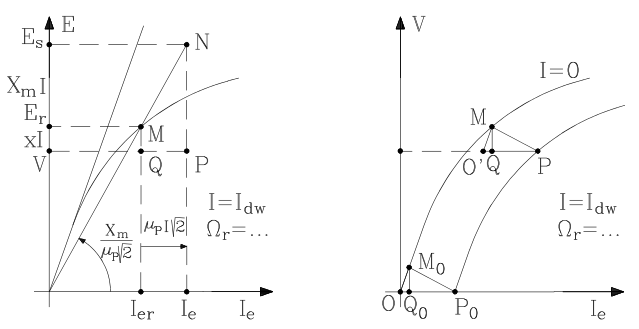
\includegraphics[scale=0.5]{ch7/image8.png}
		\captionof{figure}{La triangle $QMP$ est constant pour une valeur de $I$}
		\end{center}
		Dans le cas d'un court-circuit ($V=0$) on peut obtenir deux relations 
		intéressantes (math non détaillées ici) :
		\begin{equation}
		OP_0 = I_e = Q_0P_0\dfrac{x+X_{m,ns}}{X_{m,ns}}
		\end{equation}
		\begin{equation}
		OQ_0 = \dfrac{x}{X_{m,ns}}Q_0P_0
		\end{equation}
		L'intérêt est de pouvoir donner la caractéristique \textbf{complète} en 
		déwatté par déplacement vertical $MQ$ et horizontal $QP$. Voir page 7.23 
		pour les détails
		
		
	\subsection{Application : la caractéristique de régulation - méthode de Potier}
	Compléter après labo
		
		
		
		
		
		
		
		
		
		